\chapter{Kinetic plasma physics for the problem}\label{ch:plasma}

With the dark-photon field and its coupling to charges in hand, the question becomes how a plasma responds to a force of this kind, and the answer is kinetic. This chapter develops the kinetic plasma theory that the later chapters use as a yardstick. Every result of the paper is at some point compared with a linear dispersion relation, a growth rate or an exactly solvable limit, and the verification suite of Dark-SPECTRAX (the A, B and C items of the status ladder) is built from the cases below. The chapter is meant to be read once, in order, and then used as a reference. We keep to one dimension in space and velocity whenever possible, and treat the electromagnetic and relativistic cases separately when they are needed.

\section{The Vlasov--Maxwell system}\label{sec:vm}

A collisionless plasma of species $s$, with charge $q_s$ and mass $m_s$, is described by the distribution function $f_s(\bx,\bv,t)$ obeying
\begin{equation}
\pd{f_s}{t}+\bv\cdot\nabla f_s+\frac{q_s}{m_s}\big(\bE+\bv\times\bB\big)\cdot\pd{f_s}{\bv}=0 ,\label{eq:vlasov}
\end{equation}
coupled to Maxwell's equations through $\rho=\sum_sq_s\int f_s\,\dd^3v$ and $\bJ=\sum_sq_s\int\bv f_s\,\dd^3v$. The equation says that $f_s$ is constant along particle trajectories. Because the force field is divergence-free in velocity space, $\partial_{\bv}\!\cdot\!(\bE+\bv\times\bB)=0$, the flow in phase space is incompressible, which implies that every functional $\int G(f_s)\,\dd^3x\,\dd^3v$ is conserved. These Casimir invariants include the entropy and the $L^2$ norm of $f_s$. Whether a numerical method respects some of them is one of the main questions of Chapter~\ref{ch:numerics}. The Vlasov equation was introduced by Vlasov~\citep{Vlasov1968}, who obtained from it the dispersion relation of plasma oscillations; the version with the Lorentz force and the self-consistent fields is the one used here.

Multiplying Eq.~\eqref{eq:vlasov} by $\tfrac12m_sv^2$ and integrating gives the kinetic energy equation $\dot K=\int\bJ\cdot\bE\,\dd^3x$, and Poynting's theorem gives $\dot U_\gamma=-\int\bJ\cdot\bE$, so $K+U_\gamma$ is conserved in a closed or periodic domain. The conservation of this sum is the benchmark of the energy ledger described in Sec.~\ref{sec:energy}. In one dimension (variables $x$, $v_x$, with $\bE=E\hat x$) the magnetic term drops, Faraday's law is irrelevant, and Amp\`ere's law is $\epsilon_0\partial_tE=-J$ with Poisson's equation as a consistency condition. We call this the Vlasov--Amp\`ere system; it is the model solved by all the one-dimensional benchmarks.

The relativistic version replaces velocity by momentum. With $\bp$ the momentum, $\gamma=\sqrt{1+p^2/m^2c^2}$ and $\bv=\bp/(m\gamma)$,
\begin{equation}
\pd{f_s}{t}+\frac{\bp}{m_s\gamma}\cdot\nabla f_s+q_s\Big(\bE+\frac{\bp}{m_s\gamma}\times\bB\Big)\cdot\pd{f_s}{\bp}=0 .\label{eq:vlasovRel}
\end{equation}
The form is conservative in momentum space for the same reason as before: the electric force does not depend on $\bp$, and the magnetic term has $\partial_{\bp}\!\cdot\!(\bp\times\bB/\gamma)=\nabla_{\bp}(1/\gamma)\cdot(\bp\times\bB)=0$ because $\nabla_{\bp}(1/\gamma)\parallel\bp$. The distribution in momentum is the natural variable because $f\,\dd^3p$ is the number density in a Lorentz-invariant sense and because the kinetic term has no $\gamma$ in the force. The current is $\bJ=\sum_sq_s\int\bp f_s/(m_s\gamma)\,\dd^3p$ and the kinetic energy is $K=\sum_s\int(\gamma-1)m_sc^2f_s\,\dd^3x\,\dd^3p$.

\section{Linear theory: dielectric function, plasma dispersion function, Landau damping}\label{sec:linear}

Take a spatially uniform equilibrium $f_0(v)$ (normalized to unit density) and a perturbation $f_1\propto\ee^{\ii(kx-\omega t)}$ with the electrostatic field $E_1$ of the same dependence. In one dimension the linearized Vlasov equation is $-\ii(\omega-kv)f_1=-(q/m)E_1\,\partial_vf_0$, hence
\begin{equation}
f_1=-\ii\,\frac{q}{m}\,\frac{E_1\,\partial_vf_0}{\omega-kv} .\label{eq:f1}
\end{equation}
Poisson's equation $\ii k\epsilon_0E_1=q n_0\int f_1\,\dd v$ then determines the field self-consistently: $\ii kE_1=-\ii\,(q^2n_0/m\epsilon_0)\,E_1\int\partial_vf_0/(\omega-kv)\,\dd v$, so a nonzero $E_1$ requires
\begin{equation}
\epsilon(k,\omega)\equiv1-\frac{\omega_p^2}{k^2}\int\frac{\partial_vf_0}{v-\omega/k}\,\dd v=0 ,\qquad \omega_p^2=\frac{n_0q^2}{\epsilon_0m} ,\label{eq:eps}
\end{equation}
where we divided by $k$ and wrote $\omega-kv=-k(v-\omega/k)$. For several species the second term is summed over species. A check is the cold limit $f_0=\delta(v)$: integrating by parts, $\int\delta'(v)/(v-\omega/k)\,\dd v=1/(\omega/k)^2$, so $\epsilon=1-\omega_p^2/\omega^2$ and the root is the plasma frequency. A cold plasma has no dependence on $k$.

The integral in Eq.~\eqref{eq:eps} has a pole at $v=\omega/k$ on the real axis. Landau showed that the correct treatment of the initial-value problem requires the Laplace transform in time and that the dispersion relation for modes with $\Imag\,\omega<0$ is the analytic continuation from $\Imag\,\omega>0$~\citep{Landau1946}. The resulting prescription is that the integration contour in $v$ passes below the pole when $\Imag\omega>0$ and is deformed accordingly when $\omega$ moves into the lower half plane; on the real axis it amounts to the Plemelj formula, $1/(v-w)\to\mathrm{P}/(v-w)+\ii\pi\,\mathrm{sgn}(\Imag w)\,\delta(v-w)$. For a Maxwellian with thermal speed $\vte^2=T/m$, $f_0=\ee^{-v^2/2\vte^2}/(\sqrt{2\pi}\,\vte)$, we have $\partial_vf_0=-(v/\vte^2)f_0$. Let $\zeta=\omega/(\sqrt2k\vte)$ and $u=v/(\sqrt2\vte)$. The plasma dispersion function of Fried and Conte~\citep{FriedConte1961},
\begin{equation}
Z(\zeta)=\frac{1}{\sqrt\pi}\int_{C}\frac{\ee^{-u^2}}{u-\zeta}\,\dd u ,\label{eq:Z}
\end{equation}
with $C$ the Landau contour, gives $\int f_0/(v-w)\,\dd v=Z(\zeta)/(\sqrt2\vte)$ and so $\int\partial_vf_0/(v-w)\,\dd v=-(1+\zeta Z)/\vte^2$, using $\int vf_0/(v-w)\,\dd v=1+w\int f_0/(v-w)\,\dd v$. The dielectric function of a Maxwellian plasma is thus
\begin{equation}
\epsilon(k,\omega)=1+\frac{1}{k^2\lDe^2}\big[1+\zeta Z(\zeta)\big] ,\qquad\lDe=\frac{\vte}{\wpe} ,\label{eq:epsMax}
\end{equation}
the form used in the verification of the Hermite code, where the SciPy Faddeeva function supplies $Z$ via $Z(\zeta)=\ii\sqrt\pi\,w(\zeta)$. The code checks the complex roots of Eq.~\eqref{eq:epsMax} against the fitted frequency and damping of the Hermite solver for $k\lDe=0.2$--$0.7$, and the worst relative error over 32 runs is $1.3\times10^{-4}$ (docs/results.md, B00; the damping at $k\lDe=0.2$ is $\sim5\times10^{-5}$ and is not resolved in the fit window, so only the frequency is validated there).

For $\zeta\gg1$ the asymptotic expansion $Z(\zeta)\simeq-\zeta^{-1}(1+\tfrac12\zeta^{-2}+\tfrac34\zeta^{-4})+\ii\sqrt\pi\,\ee^{-\zeta^2}$ gives $1+\zeta Z\simeq-\tfrac12\zeta^{-2}-\tfrac34\zeta^{-4}+\ii\sqrt\pi\,\zeta\,\ee^{-\zeta^2}$. The real part of $\epsilon=0$ is then $1-\wpe^2/\omega^2-3k^2\vte^2\wpe^2/\omega^4=0$ (using $2\zeta^2=\omega^2/k^2\vte^2$), so to the first order in $k^2\lDe^2$
\begin{equation}
\omega^2=\wpe^2+3k^2\vte^2 ,\label{eq:BG}
\end{equation}
the Bohm--Gross dispersion relation for Langmuir waves~\citep{BohmGross1949}. The factor 3 is the effective adiabatic index of a one-dimensional gas, since the wave is too fast for heat to be exchanged by streaming. The imaginary part gives the damping rate by the usual perturbative argument, $\gamma=-\Imag\epsilon/(\partial\Real\epsilon/\partial\omega)$. With $\partial_\omega\Real\epsilon\simeq2/\wpe$ and $\zeta^2\simeq1/2k^2\lDe^2+3/2$,
\begin{equation}
\gamma_L=-\sqrt{\frac\pi8}\,\frac{\wpe}{(k\lDe)^3}\exp\Big[-\frac{1}{2k^2\lDe^2}-\frac32\Big] ,\label{eq:landau}
\end{equation}
which is Landau's result~\citep{Landau1946}. The origin of the damping is the resonant interaction with particles whose velocity is near the phase velocity $\omega/k$: where $\partial_vf_0<0$ at the resonance there are more particles slightly slower than the wave than faster, and the net energy flows from the wave to the particles. Landau damping is collisionless but not reversible in the usual sense: the energy goes into the distribution function as a fine-scale structure in velocity, $\ee^{-\ii kvt}$ in phase, and the field decays while the information is stored in $f_1$. This is the origin of the filamentation of phase space, and it explains why the closure of a Hermite expansion is a delicate matter (Sec.~\ref{sec:hermite}): a finite number of Hermite functions cannot hold a structure whose velocity scale shrinks as $1/t$.

For the plasma of ions and electrons the same calculation applies to each species. In Dark-SPECTRAX the dark photon modifies the kernel, and the longitudinal dispersion relation becomes $D_L=(Q-\OmD^2)(1+\chi_e)+\eta^2Q\chi_e$ with $\chi_e=k^{-2}\lDe^{-2}(1+\zeta Z)$ and $Q=\omega^2-k^2c^2$ (Sec.~\ref{sec:coupling}); its roots are what B00 compares against.

\section{Beams, ion sound and anisotropy}\label{sec:instab}

Landau damping removes energy from a wave when $f_0$ decreases at the resonant velocity, and an increasing slope reverses the sign. The simplest instance is the two-stream instability of two cold equal counter-streaming beams, each of density $n_0/2$ and velocity $\pm u$. The dispersion relation is $1=\tfrac12\wpe^2[(\omega-ku)^{-2}+(\omega+ku)^{-2}]$. With $x=\omega^2$ and $a=ku$ it becomes $(x-a^2)^2=\wpe^2(x+a^2)$, a quadratic whose roots are $x=\tfrac12[(2a^2+\wpe^2)\pm\wpe\sqrt{\wpe^2+8a^2}]$. The lower root is negative for $a<\wpe$, so $\omega$ is purely imaginary there. Writing $s=a^2/\wpe^2$, $x/\wpe^2=\tfrac12[(2s+1)-\sqrt{1+8s}]$ has its minimum at $\sqrt{1+8s}=2$, that is $s=3/8$, where $x=-\wpe^2/8$:
\begin{equation}
\gamma_{\max}=\frac{\wpe}{2\sqrt2}\qquad\text{at}\qquad ku=\sqrt{3/8}\,\wpe .
\end{equation}
Thermal spread in each beam reduces the growth and eventually removes it when the velocity spread is comparable to the beam velocity. The bump-on-tail case is the same instability for a weak beam: the growth rate is the Landau damping rate with the sign of $\partial_vf_0$ reversed at the velocity of the beam, and both cases are run as benchmark B02/B03 with the growth compared with the kinetic roots (status ladder; the mixing with a dark photon raises the growth by a few per cent in the README records).

Ion-acoustic waves exist because the heavy ions carry the inertia and the light electrons the pressure. For $\omega\ll k\vte$ the electrons are close to Boltzmann, $\chi_e\simeq1/(k\lDe)^2$, and the cold ion response is $-\wpi^2/\omega^2$, so
\begin{equation}
1+\frac{1}{k^2\lDe^2}-\frac{\wpi^2}{\omega^2}=0\quad\Rightarrow\quad\omega^2=\frac{k^2c_s^2}{1+k^2\lDe^2},\qquad c_s^2=\frac{T_e}{m_i},
\end{equation}
because $\wpi^2\lDe^2=T_e/m_i$. The wave is weakly damped only if the ions are cold: with ion thermal speed comparable to $c_s$ there are many ions at the phase velocity and ion Landau damping is strong. The standard small-damping estimate is $|\gamma/\omega|\simeq\sqrt{\pi/8}\,[\sqrt{m_e/m_i}+(T_e/T_i)^{3/2}\ee^{-T_e/2T_i-3/2}]$~\citep{Stix1992}, which is of order unity at $T_e=T_i$. The case $T_i=T_e$ is the one of HHS and of the cosmological plasma, and it matters for the argument of Sec.~\ref{sec:parametric}: ion-acoustic waves are strongly damped, so a purely growing instability that relies on them must exceed their damping before it can act.

The Buneman instability is the case of an electron beam of velocity $u$ drifting through ions. In the cold fluid model $1-\wpi^2/\omega^2-\wpe^2/(\omega-ku)^2=0$. Take $ku=\wpe$ and $\omega=\wpe\,\delta$ with $|\delta|\ll1$; then $\wpe^2/(\omega-ku)^2\simeq1+2\delta$ and the dispersion relation reduces to $\wpi^2/\omega^2=-2\omega/\wpe$, that is $\omega^3=-\tfrac12\wpi^2\wpe$. One root has positive imaginary part,
\begin{equation}
\gamma=\frac{\sqrt3}{2}\Big(\frac{m_e}{2m_i}\Big)^{1/3}\wpe\simeq0.056\,\wpe\qquad(m_i/m_e=1836),
\end{equation}
the result of Buneman~\citep{Buneman1958}. The Dark-SPECTRAX records for $m_i/m_e=100$ and $1836$, ordinary and dark, agree with the kinetic roots to $1.5\times10^{-4}$ (B05).

The Weibel instability is the electromagnetic instability of a plasma with an anisotropic temperature, $T_\perp>T_\parallel$ in the direction of the wave vector. For a bi-Maxwellian the transverse dispersion relation is $\omega^2-k^2c^2-\wpe^2+\wpe^2(T_\perp/T_\parallel)[1+\zeta Z(\zeta)]=0$ with $\zeta=\omega/(\sqrt2k v_\parallel)$ and $v_\parallel^2=T_\parallel/m$. At marginal stability $\omega\to0$, $\zeta Z\to0$, and $k^2c^2=\wpe^2(T_\perp/T_\parallel-1)\equiv\wpe^2A$, so the unstable band is $k<k_c=\sqrt A\,\wpe/c$. For $\omega=\ii\gamma$ with $\gamma\ll kv_\parallel$, $Z\simeq\ii\sqrt\pi$, so $1+\zeta Z\simeq1-\sqrt{\pi/2}\,\gamma/(kv_\parallel)$ and the dispersion relation gives
\begin{equation}
\gamma=\sqrt{\frac{2}{\pi}}\;kv_\parallel\,\frac{A-k^2c^2/\wpe^2}{1+A} ,
\end{equation}
which is Weibel's growth rate~\citep{Weibel1959} in the regime of its validity. Dark-SPECTRAX reproduces this and the related filamentation instability of counter-streaming beams in 1D3V at $k=0.4$--$2.4$ to within $10^{-3}$ for ordinary and dark runs (B09), at the price of $N_n=512$ at the largest $k$. The point of the Weibel and Buneman tests is not that they matter for the cosmological problem; it is that they exercise the electromagnetic and ion-electron parts of the kernel against exact answers.

\section{Nonlinear phenomena: echoes, trapping, Langmuir turbulence}\label{sec:nonlinear}

Landau damping is a statement about the linear equations, and its reversibility is shown by the plasma-wave echo~\citep{Gould1967}. Apply a density perturbation of wave number $k_1$ at $t=0$ and another of $k_2$ at $t=\tau$. After each, the field decays by phase mixing. The first perturbation leaves $f_1\propto\ee^{\ii k_1(x-vt)}g(v)$; at $t=\tau$ the field of the second kicks the distribution through $E_2\partial_v$, and the product of the second kick with the $-k_1$ component of the first (carrying velocity dependence $\ee^{+\ii k_1v\tau}$) generates a component with wave number $k_3=k_2-k_1$ whose velocity phase is $\ee^{\ii k_1v\tau}\ee^{-\ii k_3v(t-\tau)}$. The phase is independent of $v$, so the macroscopic density does not cancel, at
\begin{equation}
t_{\rm echo}=\tau\,\frac{k_2}{k_2-k_1}.
\end{equation}
The benchmark B06 uses $k_1=1$, $k_2=1.5$, $\tau=10$, so $t_{\rm echo}=30$; the Hermite echo amplitude matches an independent grid solver to $2\times10^{-5}$ (ordinary) and $1.6\times10^{-5}$ (dark). Mixing with the dark photon lowers the echo by $3.3\%$ (README, B06 record). The echo shows that the information lost by Landau damping is in the fine velocity structure of $f_1$, and therefore it also shows why the Hermite method must either hold that structure or filter it, with a consequent loss of the reversibility.

When the wave amplitude is large, linear theory fails because particles are trapped. A particle in a wave of amplitude $E$ and phase velocity $v_\phi=\omega/k$ obeys, in the wave frame, a pendulum equation, $\ddot\theta=-(qkE/m)\sin\theta$ with $\theta=kx-\omega t$, so trapped particles bounce at $\omega_b=\sqrt{qkE/m}$ within a velocity width $\Delta v=2\omega_b/k$ around $v_\phi$. Once $\omega_b$ exceeds the linear damping rate, the particles complete several bounce periods before the wave has damped, the distribution flattens at the resonance (a plateau forms) and damping is switched off; the field then oscillates with the bounce period around a finite amplitude. This is the picture of O'Neil~\citep{ONeil1965}, who solved the nonlinear problem of a wave whose amplitude varies slowly compared to the bounce period and found that the rate of damping drops with time as the plateau forms, and that the electric field then undergoes oscillations with amplitude and period set by the bounce frequency. The Dark-SPECTRAX benchmark B01 follows nonlinear Landau damping at $k\lDe=0.3$ and $\delta n/n=0.05$, where the rebound of the envelope is on the bounce time scale; the repository records the field history against the grid solvers, and the dark trapping minimum arrives earlier than the ordinary one ($t=30.5$ against $31.45$; README, B01 record).

Langmuir waves interact with ion density fluctuations through the ponderomotive force. For a high-frequency field $\tfrac12(\mathcal E\,\ee^{-\ii\omega_pt}+\mathrm{c.c.})$ with slowly varying envelope $\mathcal E$, an electron feels the time-averaged force $-\nabla\Phi_p$ with $\Phi_p=e^2|\mathcal E|^2/(4m\omega_p^2)=\epsilon_0|\mathcal E|^2/(4n_0)$, using $\omega_p^2=n_0e^2/\epsilon_0m$. The electron fluid transmits this force to the ions through the ambipolar field, and the low-frequency density response $\delta n$ obeys the driven ion-acoustic equation. Together with the envelope equation obtained from the Bohm--Gross relation, $\omega\simeq\omega_p(1+\delta n/2n_0+\tfrac32k^2\lDe^2)$ and $k\to-\ii\nabla$, one has the Zakharov equations~\citep{Zakharov1972}:
\begin{align}
\ii\,\partial_t\mathcal E+\tfrac32\,\omega_p\lDe^2\nabla^2\mathcal E&=\tfrac12\,\omega_p\,\frac{\delta n}{n_0}\,\mathcal E ,\label{eq:zakE}\\
\big(\partial_t^2-c_s^2\nabla^2\big)\frac{\delta n}{n_0}&=\frac{\epsilon_0}{4m_in_0}\,\nabla^2|\mathcal E|^2 .\label{eq:zakN}
\end{align}
The first describes Langmuir waves whose frequency is shifted by the local density, and the second the ion density driven by the ponderomotive force. A uniform Langmuir wave that is modulated in space finds that regions of high field amplitude expel plasma and the lower density in the region traps more field, so the modulation grows. Zakharov showed that when the energy density of the Langmuir field exceeds $nT(k r_D)^2$ the system collapses~\citep{Zakharov1972}. The simplest consequence of Eqs.~\eqref{eq:zakE}--\eqref{eq:zakN} is the modulational instability of a uniform Langmuir wave of amplitude $\mathcal E_0$. When the ions respond quasi-statically, $\partial_t^2\ll c_s^2\nabla^2$ in Eq.~\eqref{eq:zakN}, the density perturbation follows the field, $\delta n/n_0=-\epsilon_0|\mathcal E|^2/(4n_0T_e)$, because $c_s^2m_i=T_e$. Equation~\eqref{eq:zakE} then becomes the nonlinear Schr\"odinger equation $\ii\partial_t\mathcal E+P\nabla^2\mathcal E+Q|\mathcal E|^2\mathcal E=0$ with $P=\tfrac32\omega_p\lDe^2$ and $Q=\omega_p\epsilon_0/(8n_0T_e)$, both positive, which is the focusing case. Write $\mathcal E=(\mathcal E_0+\delta)\ee^{\ii Q\mathcal E_0^2t}$ and linearize in a small complex $\delta\propto\ee^{\ii Kx+\gamma t}$ and its conjugate. The result is $\gamma^2=P K^2(2Q\mathcal E_0^2-PK^2)$, so a plane wave is unstable to modulations with $K^2<2Q\mathcal E_0^2/P$; the growth rate is largest at $K^2=Q\mathcal E_0^2/P$, where
\begin{equation}
\gamma_{\max}=Q\mathcal E_0^2=\frac{\omega_p}{2}\,\frac{\epsilon_0\mathcal E_0^2}{4n_0T_e} .
\end{equation}
The growth rate is a fraction of the plasma frequency set by the ratio of the Langmuir energy density to the thermal energy density, which is the origin of the statement that nonlinearity matters when the wave energy approaches the thermal energy. The inclusion of ion inertia and of kinetic ion Landau damping, which at $T_i=T_e$ cannot be ignored, lowers it, and the B10 benchmark checks which of these corrections survive in the Hermite model.

Equations~\eqref{eq:zakE}--\eqref{eq:zakN} describe the mechanism that HHS invoke when they say that a large-amplitude $k=0$ Langmuir wave produces density inhomogeneities which detune the resonance, and they are the origin of the B10 benchmark of the repository: a finite-amplitude Langmuir pump with a single sideband pair, compared with the Zakharov growth rate and a semi-kinetic version in which the exact dispersion relation and kinetic ions are used. The two checks bracket the question, because the Zakharov limit assumes $k\lDe\ll1$ and fluid ions, while at $T_i=T_e$ the ion response is strongly kinetic.

\section{Parametric instabilities of a uniform pump}\label{sec:parametric}

The dark photon acts, to leading order, as a spatially uniform oscillating electric field of frequency $\omega_0$ close to $\wL$. In the plasma physics literature this is the dipole approximation to a pump wave, and the instabilities it drives were worked out by Silin~\citep{Silin1965} in the kinetic theory and by Nishikawa~\citep{Nishikawa1968a,Nishikawa1968b} with a coupled-mode formulation. We derive the structure of the result in a fluid model that is simple enough to follow and complete enough to show the two branches.

Let the electrons oscillate in the pump with velocity $v_{\rm os}(t)$ and displacement $\xi(t)=r\cos\omega_0t$ (we drop the sign), $v_{\rm os}=r\omega_0$. In the frame moving with the oscillation, $x\to x-\xi(t)$, the electron equations contain no pump force, while the ion response at fixed $x$ acquires a phase $\ee^{\ii k\xi(t)}$ in Fourier space. Linearize about the uniform state, with electron density amplitude $N_e$, ion density amplitude $N_i$, pressure term $3\vte^2$ (adiabatic) and cold ions. The electron fluid equations $\dot N_e+\ii kn_0U=0$ and $\dot U=-(e/m)\hat E-3\ii k\vte^2N_e/n_0$ close with Poisson's equation in the moving frame, $\epsilon_0\ii k\hat E=-eN_e+eN_i\,\ee^{\ii k\xi(t)}$, which carries the pump through the phase of the ion density. Eliminating $U$ and $\hat E$,
\begin{equation}
\ddot N_e+\omega_k^2N_e=\wpe^2\,\ee^{\ii k\xi(t)}N_i ,\qquad \omega_k^2=\wpe^2+3k^2\vte^2 ,\label{eq:pumpE}
\end{equation}
and in the same way the ion equation $\ddot N_i=-\ii kn_0(e/m_i)E_x$, with $E_x=\hat E\,\ee^{-\ii k\xi}$, gives
\begin{equation}
\ddot N_i+\wpi^2N_i=\wpi^2\,\ee^{-\ii k\xi(t)}N_e .\label{eq:pumpI}
\end{equation}
Without the pump ($\xi=0$) these are the coupled Langmuir and ion-acoustic oscillators. With it the coefficients are periodic, with the Jacobi--Anger expansion $\ee^{\ii k\xi}=\sum_l\ii^lJ_l(K)\ee^{\ii l\omega_0t}$, $K\equiv kr$. Seek a Floquet solution in which $N_i\propto\ee^{-\ii\omega t}$ with slowly varying $\omega$. Equation~\eqref{eq:pumpE} gives the electron response as a sum of sidebands at $\omega-l\omega_0$,
\begin{equation}
N_e=\sum_l\ii^lJ_l(K)\,\frac{\wpe^2}{\omega_k^2-(\omega-l\omega_0)^2}\,\ee^{-\ii(\omega-l\omega_0)t}N_i .
\end{equation}
Insert this in Eq.~\eqref{eq:pumpI}, multiply by $\ee^{-\ii k\xi}=\sum_m(-\ii)^mJ_m(K)\ee^{\ii m\omega_0t}$ and keep the secular terms, those with $m=-l$ after using $J_{-l}=(-1)^lJ_l$. The product of coefficients is $\ii^l\ii^{l}(-1)^l\to J_l^2$, so the dispersion relation of the pumped system is
\begin{equation}
\omega^2-\wpi^2+\wpi^2\wpe^2\sum_{l=-\infty}^{\infty}\frac{J_l^2(K)}{\omega_k^2-(\omega-l\omega_0)^2}=0 .\label{eq:floquet}
\end{equation}
This is the Silin--Nishikawa structure in a fluid dress: a single equation for the low-frequency ion-acoustic mode, with the electron response resolved into sidebands coupled by Bessel functions of the excursion parameter $K=kr$. Without the pump only $l=0$ remains and the equation is the ion-acoustic dispersion relation, $\omega^2\simeq\omega_s^2=3k^2\vte^2m_e/m_i$ for $\omega\ll\omega_k$ (the factor 3, instead of 1 for isothermal electrons, comes from the high-frequency treatment of the electron pressure, which a kinetic electron response replaces).

For a weak pump, $K\ll1$, keep $J_0^2\simeq1-K^2/2$ and $J_{\pm1}^2\simeq K^2/4$. For $|\omega|\ll\omega_0$ the two sidebands are equal to $\omega_k^2-\omega_0^2$, and Eq.~\eqref{eq:floquet} reduces to
\begin{equation}
\omega^2=\omega_s^2-\frac{K^2}{2}\,\frac{\wpi^2\wpe^2\,\omega_0^2}{\omega_k^2(\omega_k^2-\omega_0^2)} .\label{eq:otsi}
\end{equation}
The sign of the second term is fixed by that of $\omega_k^2-\omega_0^2$. For $\omega_0<\omega_k$, a pump below the local Langmuir frequency, the pump lowers $\omega^2$ and, when the second term exceeds $\omega_s^2$, makes it negative: the root is purely imaginary, a \emph{purely growing} mode, with no frequency in the frame of the ions. This is the oscillating two-stream instability (OTSI) of Nishikawa~\citep{Nishikawa1968a}. For $\omega_0>\omega_k$ the term is positive and no purely growing root exists. Instead, when $\omega_0-\omega_k\simeq\pm\omega_s$ one sideband is resonant, the corresponding denominator in Eq.~\eqref{eq:floquet} is small, and the root is a complex pair of the parametric decay instability (PDI), in which the pump decays into a Langmuir wave and an ion-acoustic wave with $\omega_0=\omega_k+\omega_s$. The two branches are the two sides of the pump frequency relative to $\omega_k(k)$, and they are the two sides, for a resonant pump close to $\wpe$, of the Langmuir dispersion curve.

The scaling of the purely growing branch follows from Eq.~\eqref{eq:otsi}. For $\gamma^2=-\omega^2$ well above threshold,
\begin{equation}
\gamma\simeq\frac{kr}{\sqrt2}\,\frac{\wpi\wpe\,\omega_0}{\omega_k\sqrt{\omega_k^2-\omega_0^2}} ,\qquad kr=\frac{kv_{\rm os}}{\omega_0}.
\end{equation}
At the resonance $\omega_0\simeq\wpe$ the denominator is $\omega_k^2-\omega_0^2\simeq3k^2\vte^2$, and the $k$ cancels:
\begin{equation}
\gamma_{\rm OTSI}\simeq\frac{\wpi}{\sqrt6}\,\frac{v_{\rm os}}{\vte}.\label{eq:gammaOTSI}
\end{equation}
The growth is broadband in $k$, proportional to the ion plasma frequency and to the oscillation speed measured in thermal speeds, and independent of the wave number as long as the weak-pump and long-wavelength assumptions hold. It is set by the same ratio that defines the drive in the simulations: for a resonant pump $v_{\rm os}$ grows secularly as $E_0t/2$, so the OTSI growth rate rises linearly with time and the instability appears when it overcomes the damping of the ion wave, here the ion Landau damping at $T_i=T_e$, which the fluid-ion model does not contain. The kinetic version changes the numerical factor and adds the damping, and the Floquet analysis of the Hermite model reproduces the kinetic dipole-pump determinant of Silin to $1.3\%$ at 22 unstable points, with growth rates that vanish with fixed ions, are purely growing and vanish on the decay side (README, OTSI section; docs/results.md). We checked Eq.~\eqref{eq:floquet} for $\omega_0$ below $\omega_k$ by solving it numerically for several $K\le0.2$: the purely imaginary root appears above threshold and Eq.~\eqref{eq:otsi} gives its order of magnitude, overestimating $\gamma$ when $\omega_k-\omega_0$ is comparable to $\gamma$ (the sidebands are then not far from resonance and the approximation $|\omega|\ll\omega_k-\omega_0$ fails).

This is the physical content of the argument by HHS that large-amplitude Langmuir waves excite higher-$k$ Langmuir and ion-acoustic waves. In the language used here, the electrons oscillate with an excursion that grows in time, the uniform pump becomes a modulation of the ion density through the factor $\ee^{\ii k\xi}$, and the OTSI feeds a broadband spectrum at all $k$ for which the ion-wave damping is weaker than $\gamma_{\rm OTSI}$. The paper's question is then whether this instability, which exists in the model, is what limits the transfer in the HHS configuration, or whether it is limited by another mechanism earlier; the relativistic detuning of Sec.~\ref{sec:relativistic} gives the second answer.

\section{Collisions}\label{sec:collisions}

The ordinary collision operator of plasma physics is the Landau (or Fokker--Planck) operator, which is a nonlinear integro-differential operator in velocity space. The simplest model that retains the main effects is the Lenard--Bernstein operator~\citep{LenardBernstein1958},
\begin{equation}
C[f]=\nu\,\pd{}{v}\Big[(v-u)f+v_t^2\pd{f}{v}\Big] ,\label{eq:LB}
\end{equation}
with a velocity-independent frequency $\nu$, which diffuses $f$ in velocity and drags it towards the velocity $u$ with a diffusion coefficient $\nu v_t^2$. Dougherty~\citep{Dougherty1964} made it conservative by taking the flow velocity $u$ and the temperature $v_t^2=T/m$ to be those of $f$ itself, so that number, momentum and energy are conserved exactly, while the only equilibrium is the Maxwellian. The operator is a single-species model and is accurate for the bulk of the distribution but not for the tail; the multispecies generalization is, in Dougherty's words, similar in principle and more cumbersome.

Hermite functions diagonalize the operator. Take $u=0$ and write $v=\sqrt2\,v_t\xi$, so that Eq.~\eqref{eq:LB} becomes $\nu\,\partial_\xi(\xi f+\tfrac12\partial_\xi f)$. For $f=H_n(\xi)\ee^{-\xi^2}$ one has $\xi f+\tfrac12\partial_\xi f=\tfrac12H_n'\ee^{-\xi^2}$, and applying $\partial_\xi$ and the Hermite equation $H_n''-2\xi H_n'=-2nH_n$,
\begin{equation}
C\big[H_n\ee^{-\xi^2}\big]=-n\nu\,H_n\ee^{-\xi^2} .\label{eq:LBhermite}
\end{equation}
The mode of order $n$ in the Hermite basis matched to the Maxwellian relaxes at the rate $n\nu$, so $n=0$ (density) is conserved and $n=1,2$ (momentum and energy) are protected by the corrections that make the operator conservative. The damping that grows linearly with $n$ acts as a physical filter of the fine velocity structure that Landau damping produces, and it is the physical analogue of the artificial hypercollisions used as closures (Sec.~\ref{sec:hermite}). In a basis with a different width or centre, the operator also couples neighbouring orders, which Hakim et al.~\citep{Hakim2020} treat in a conservative discretization; this is the version used in the repository.

For several species, the cross-species terms need a choice. Francisquez et al.~\citep{Francisquez2022} give a general family: the species-$s$ operator with $r$ uses a cross drift $u_{sr}$ and cross temperature $T_{sr}$ that must be chosen so that momentum and energy are conserved in the exchange and the exchange reproduces the known relaxation rates of the Fokker--Planck operator. One choice, which we call LBO-EM, takes the arithmetic mean of the two flow speeds and a common temperature; with it the momentum exchange rate equals the Morse rate and the temperature-difference rate equals twice the Morse rate. The choice due to Greene~\citep{Greene1973} (LBO-G), with parameter $\beta=0$, makes both rates equal to the Morse rates. The repository implements both (the pull requests numbered 71 and 73 of the parent), verifies momentum and energy conservation to round-off, and verifies exchange rates against exact solutions to $10^{-13}$ (B11). The collision frequencies are velocity independent, $\nu_{ee}=\nu_{ei}$, $\nu_{ii}=\nu_{ei}\sqrt{m_e/m_i}$ and $m_e\nu_{ei}=m_i\nu_{ie}$.

The constancy of $\nu$ is the weakest point of the model for the cosmological application, because the real electron--ion collision frequency depends on the energy as $v^{-3}$. The Spitzer frequency~\citep{Spitzer1962,Braginskii1965} is
\begin{equation}
\nu_{ei}=\frac{4\sqrt{2\pi}}{3}\,\frac{n_iZ^2e^4\ln\Lambda}{(4\pi\epsilon_0)^2\,m_e^{1/2}\,T_e^{3/2}} ,
\end{equation}
which falls as $T_e^{-3/2}$: an electron population heated by the resonance becomes less collisional, which is a positive feedback for collisionless physics and a reason why the constant-$\nu$ calculation is a first step and not a cosmological calculation.

\section{The driven oscillator and Drude absorption}\label{sec:drude}

When collisions act on a plasma driven at the plasma frequency they limit the build-up of the resonance. A simple model with drag $\nu$ captures the effect: the electron fluid obeys $\dot v=-(e/m)(E+E_{\rm dr})-\nu v$, so that, with $\epsilon_0=1$, $\dot J=-\nu J+\wpe^2(E+E_{\rm dr})$ and $\dot E=-J$. For $E_{\rm dr}=\Real\,E_0\ee^{-\ii\omega t}$ the steady state is
\begin{equation}
J=\frac{\wpe^2\omega\,E_0}{\nu\omega-\ii(\omega^2-\wpe^2)} ,
\end{equation}
as follows from $E=-\ii J/\omega$, and the time-averaged power absorbed from the drive is
\begin{equation}
P=\tfrac12\Real(JE_0^*)=\frac{\wpe^2\nu\,\omega^2\,E_0^2}{2\,[(\omega^2-\wpe^2)^2+\nu^2\omega^2]} .\label{eq:drude}
\end{equation}
At resonance $P=\wpe^2E_0^2/(2\nu)$: the absorption is larger the lower the collision rate, provided the steady state is reached, which requires $\nu t\gtrsim1$. The repository finds that kinetic collisional absorption in the Dougherty model follows this law with $\nu_{\rm eff}=\tfrac12\nu_{ei}(1+m_e/m_i)$ (the value in the paper, Sec. on collisional absorption). With ions included the plasma frequency is $\wL$. In the collisionless limit $\nu\to0$ Eq.~\eqref{eq:drude} becomes a delta function in $\omega$, and the response is not a steady state but the secular growth derived in Sec.~\ref{sec:resonance}.

\section{Relativistic dynamics and why the resonance switches off}\label{sec:relativistic}

A resonantly driven oscillator can leave its resonance because its frequency depends on its amplitude. In a plasma the electron mass is $\gamma m$, and the mass increases with the quiver speed, so the oscillation frequency decreases. We derive the effect in the cold, uniform case, where the electrons move with the single momentum $p(t)$. In units $c=\wpe=n=m=1$ the equations are $\dot p=-F$ with $F=E+E_{\rm dr}$, the force field, and $\dot E=-J=p/\gamma$ for electrons of charge $-1$ and $\gamma=\sqrt{1+p^2}$ (the ions only add the small term of Sec.~\ref{sec:resonance}). Without the drive, $\ddot p=-p/\sqrt{1+p^2}\simeq-p+\tfrac12p^3$. This is a Duffing oscillator with a softening nonlinearity, whose frequency for amplitude $p_0$ follows from the Lindstedt expansion, $\omega=1+\tfrac38\beta p_0^2$ with $\beta=-\tfrac12$ the coefficient of the cubic term:
\begin{equation}
\omega=\wpe\Big(1-\tfrac{3}{16}\,p_0^2\Big) .\label{eq:duffing}
\end{equation}
The relative frequency shift, $-\tfrac3{16}v^2/c^2$, is the cold relativistic shift of the Langmuir oscillation known since Akhiezer and Polovin~\citep{AkhiezerPolovin1956}.

Now include the drive. Write $p=\Real(Pe^{-\ii t})$, $E=\Real(\mathcal Ee^{-\ii t})$ and $E_{\rm dr}=E_0\cos t$ (the difference between $\wL$ and $\wpe$ is a fraction $m_e/2m_i$ and is ignored here). To the order of the first harmonic, $p/\gamma\simeq p-\tfrac12p^3$ is represented by $P-\tfrac38|P|^2P$. The slow equations are
\begin{equation}
\dot P-\ii P=-\mathcal E-E_0 ,\qquad \dot{\mathcal E}-\ii\mathcal E=P-\tfrac38|P|^2P .
\end{equation}
Form $u=P-\ii\mathcal E$ and $w=P+\ii\mathcal E$. Subtracting $\ii$ times the second equation from the first, the large terms cancel and $\dot u=-E_0+\ii\tfrac38|P|^2P$; the combination $w$ rotates at twice the carrier and averages out, so $P\simeq u/2$ and
\begin{equation}
\dot u=-E_0+\ii\,\frac{3}{64}\,|u|^2u .\label{eq:slowflow}
\end{equation}
With $u=-r\ee^{\ii\psi}$ this is a pair of real equations,
\begin{equation}
\dot r=E_0\cos\psi ,\qquad \dot\psi=\frac{3}{64}\,r^2-\frac{E_0}{r}\sin\psi .\label{eq:slowflowReal}
\end{equation}
For small $\psi$ and $r\simeq E_0t$ the phase advances as $\dot\psi\simeq\tfrac3{64}E_0^2t^2$, so $\psi\simeq E_0^2t^3/64$. Here $r=2p_0$ and $\tfrac3{64}r^2=\tfrac3{16}p_0^2$ is the shift of Eq.~\eqref{eq:duffing}. The growth of the amplitude, $\dot r=E_0\cos\psi$, is the linear resonance law as long as $\psi\ll1$ and it stalls when the phase between the oscillation and the drive reaches $\pi/2$; the resonance is lost because the oscillator frequency has drifted away from that of the drive by an amount that accumulates as $t^2$, the signature of a secular, amplitude-driven detuning. The time scale is $t_{\rm det}\sim(64/E_0^2)^{1/3}$, which varies as $E_0^{-2/3}$. For the HHS case $E_0=\vq\,\vte\,\wpe=0.03\sqrt{10^{-3}}\simeq9.5\times10^{-4}$ in code units and $t_{\rm det}\sim4/E_0^{2/3}\simeq4\times10^2$. The external work is proportional to $r^2$, so a drop by 10\% in $\Wext$ relative to the linear law occurs when $\int\cos\psi\,\dd t$ falls by $5\%$, which is somewhat before $\psi=\pi/2$.

The cold model is not the whole story, because the plasma is not cold: the electrons have $v_{te}^2=10^{-3}c^2$, and a thermal ensemble of oscillators has its own relativistic shift. For a uniform field the current is $J=-n\langle p/\gamma\rangle$ and $\dot J=n\langle\gamma^{-3}\rangle F$, since $\partial_p(p/\gamma)=\gamma^{-3}$; the effective plasma frequency of the hot plasma is therefore $\omega_{\rm eff}^2=\wpe^2\langle\gamma^{-3}\rangle$. For a Maxwellian with $\langle p^2\rangle=\theta=\vte^2/c^2$, $\gamma^{-3}\simeq1-\tfrac32p^2$ gives $\omega_{\rm eff}\simeq\wpe(1-\tfrac34\theta)$, a constant detuning of $7.5\times10^{-4}\wpe$ for the HHS temperature. This detuning accumulates a phase of order one in a time $\sim1/\Delta\omega\simeq1.3\times10^3\wpe^{-1}$, independent of the drive, and so it dominates for weak drives, where the finite-amplitude shift of Eq.~\eqref{eq:duffing} is small. Adding both effects to Eq.~\eqref{eq:slowflowReal} as $\dot\psi=\tfrac34\theta+\tfrac3{64}r^2-(E_0/r)\sin\psi$ completes the slow-flow model.

\begin{figure}[t]
\centering
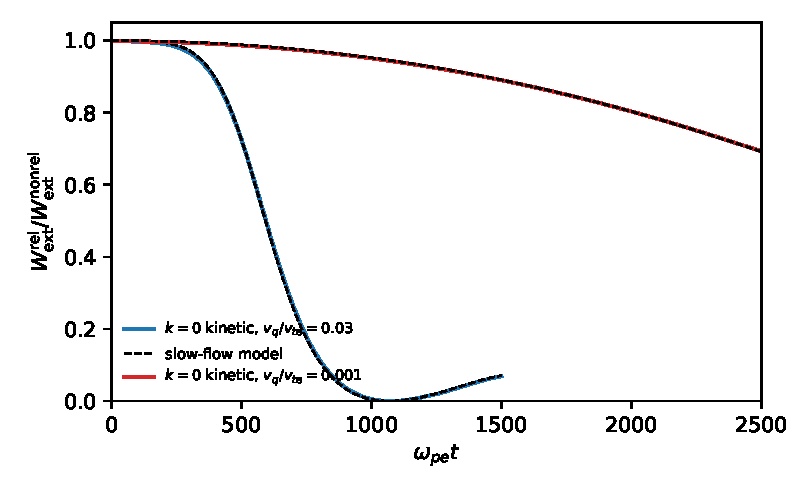
\includegraphics[width=0.78\linewidth]{figures/fig_cold_relativistic.pdf}
\caption{Ratio of the external work of the relativistic to the nonrelativistic homogeneous plasma under a resonant uniform drive (solid), from the $k=0$ Vlasov equation integrated with 48 Gauss--Hermite momentum nodes and cold ions with $m_i/m_e=1836$, and the slow-flow model with the thermal term (black dashed). Generated by \texttt{note/make\_note\_figures.py}.}\label{fig:relcold}
\end{figure}

We checked this with a calculation of our own that is exact for the homogeneous collisionless problem (script \texttt{note/make\_note\_figures.py}, output \texttt{note/figures/k0\_relativistic.json}; it is a calculation made for this note and not a study record, and it is the reference for the relativistic timing in Chapters~\ref{ch:model} and~\ref{ch:rel}): the relativistic Vlasov equation at $k=0$, in which every electron momentum evolves as $\dot p=-F(t)$ with the common force field $F$, the current is the Maxwellian average of $p/\gamma$ over the initial momentum (48 Gauss--Hermite nodes, exact for this smooth integrand to far better than the quantities quoted), and the ions are cold. Its external work departs from the nonrelativistic linear resonant law by 10\,\% at $\wpe t=392.3$ for $\vq=0.03$, against $392.5$ for the relativistic Hermite record (paper, relativistic section; \texttt{studies/relhhs/summary.json}). For $\vq=10^{-3}$ it gives $1428.8$, against $1309.5$ and $1413.5$ for the deterministic and the shot-noise relativistic grid (\texttt{studies/relgrid/summary.json}); the slow-flow model gives $397$ and $1438$. The cold model alone gives $437$ for the strong drive, and for the weak drive it does not collapse in the time of interest, which is why the thermal term is needed; the figure shows the kinetic and slow-flow results with the thermal term. We do not draw from this agreement that the detuning is the whole story of the paper's collapse time, since the continuum models include $k\neq0$ modes; but it shows that the timing of the collapse in the paper is accounted for by the homogeneous physics that nonrelativistic models cannot contain, and that no nonlinear inhomogeneous process is needed for it. This is the finding (i) of the paper's abstract. The Jüttner distribution, the relativistic equilibrium
\begin{equation}
f_J(\bp)\propto\exp\!\Big[-\frac{\gamma(p)\,mc^2}{T}\Big] ,
\end{equation}
introduced by J\"uttner~\citep{Juttner1911}, reduces to the Maxwellian when $T\ll mc^2$; in one momentum dimension its normalization is $\int\ee^{-\gamma/\theta}\dd p=2K_1(1/\theta)$ with $\theta=T/mc^2$ and $K_1$ the modified Bessel function, because with $p=\sinh s$ the integral is $2\int_0^\infty\ee^{-\cosh s/\theta}\cosh s\,\dd s$. It is the right initial condition when the electrons have been heated above a few per cent of $mc^2$.
